\documentclass{beamer}
\usepackage{amsmath}
\usepackage[utf8]{inputenc}
\usepackage{hyperref}
\usepackage{multicol}
\usepackage{hyperref}
\usepackage{xcolor}

\inputencoding{utf8}

\mode<presentation> {
    \usetheme{Madrid}
}

\usepackage{graphicx}
\usepackage{booktabs}

\title[Abstractos]{Tipos Abstractos de Datos}
\author{Ernesto Rodriguez}
\institute{
    Universidad del Itsmo \\
    \medskip \textit{erodriguez@unis.edu.gt}
}

\date[\today]{}

\begin{document}

\begin{frame}
    \maketitle
\end{frame}

\begin{frame}
\frametitle{Tipos Abstractos de Dato (ADT)}
Sea $\mathcal{S}^0:=\{\mathbb{A}_1,\ldots,\mathbb{A}_n\}$ un confjunto finito de simbolos, se
conoce a $\mathcal{S}$ como el conjunto de {\bf tipos} tal que:
\begin{itemize}
    \item{$\mathcal{S}^0\subseteq \mathcal{S}$}
    \item{Si $\mathbb{A},\mathbb{B}\in \mathcal{S}$, entonces $(\mathbb{A}\times\mathbb{B})\in\mathcal{S}$}
    \item{Si $\mathbb{A}\in\mathcal{X}$ y $\mathbb{B}\in\mathcal{S}^0$, entonces $(\mathbb{A}\rightarrow\mathbb{B})\in\mathcal{S}$}
\end{itemize}
\end{frame}

\begin{frame}
\frametitle{Tipos Abstractos de Dato}

\begin{itemize}
    \item{Si $c$ es un simbolo y $\mathbb{A}\in\mathcal{S}$, se le conoce a la pareja $[c:\mathbb{A}]$
    una {\bf declaracion de constructor} para $c$ en $\mathcal{S}$}
    \item{Si $\mathcal{S}^0$ es un conjunto de simbolos y $\mathcal{D}$ un conjunto de {\bf declaraciones
    de constructores} en $\mathcal{S}$, se conoce a la pareja $\langle \mathcal{S}^0,\mathcal{D}\rangle$
    como un {\bf Tipo abstracto de Dato}}
    \item{{\bf Ejemplo:} $\langle \{ \mathbb{B} \}, \{ [T:\mathbb{B}], [F:\mathbb{B}] \} \rangle$ es un
    tipo abstracto de dato que representa los booleanos.}
    \item{{\bf Ejemplo:} $\langle \{ \mathbb{N} \}, \{ [o:\mathbb{N}],[s:\mathbb{N}\rightarrow
    \mathbb{N}] \} \rangle$ representa los numeros naturales.}
    \item{{\bf Ejemplo:} $\langle \{ \mathbb{N}, \mathcal{L}(\mathbb{N}) \}, \{ [o:\mathbb{N}], [s:\mathbb{N}
    \rightarrow\mathbb{N}], [\mathtt{nil}:\mathcal{L}(\mathbb{N})], [\mathtt{cons}:\mathbb{N}\times
    \mathcal{L}(\mathbb{N})\rightarrow \mathcal{L}(\mathbb{N})] \} \rangle$ representa una lista
    de naturales.}
\end{itemize}

\end{frame}

\begin{frame}
\frametitle{Terminos Constructores}
Sea $\mathcal{A}:=\langle \mathcal{S}^0,\mathcal{D} \rangle$ un tipo abstracto de datos. Se conoce
el termino $t$ como un {\bf termino constructor del tipo} $\mathbb{T}$ ssi:
\begin{itemize}
    \item{$\mathbb{T}\in\mathcal{S}^0$ y $[t:\mathbb{T}\in\mathcal{D}]$ o}
    \item{$\mathbb{T}=\mathbb{A}\times\mathbb{B}$ y $t$ tiene la forma $\langle a,b \rangle$, donde
    $a$ y $b$ son constructores de los tipos $\mathbb{A}$ y $\mathbb{B}$.}
    \item{$t$ tiene la forma $c(a)$ donde $a$ es un termino constructor del tipo $\mathbb{A}$
    y hay un constructor con la declaraci\'on $[c:\mathbb{A}\rightarrow\mathbb{T}]\in\mathcal{D}$}
\end{itemize}
Se utiliza la notaci\'on $\mathcal{T}_{\mathbb{A}}^g(\mathcal{A})$ para representar el conjunto
de todos los constructores del tipo $\mathbb{A}$ y utilizamos
$\mathcal{T}^g(\mathcal{A}):=\cup_{\mathbb{A}\in\mathcal{S}}\mathcal{T}_{\mathbb{A}}^{g}(\mathcal{A})$

\end{frame}

\begin{frame}
\frametitle{Aximoas de Peano para ADTs}
\begin{itemize}
    \item{Si $t$ es un constructor del tipo $\mathbb{T}$, entonces $t\in\mathbb{T}$}
    \item{La igualdad es trivial (igualdad estructural)}
    \item{Solo los terminos constructores de $\mathbb{T}$ pertenecen al tipo $\mathbb{T}$}
\end{itemize}
\end{frame}

\begin{frame}
\frametitle{Computaci\'on mediante Constructores}
\begin{itemize}
    \item{Se desea entender la computacion de data en ADTs}
    \item{Consideremos un ejemplo concreto: $\mathcal{B}:=\langle \{\mathbb{B}\}, \{[\mathtt{T}:\mathbb{B}],
    [\mathtt{F}:\mathbb{B}]\}\rangle$ y las operaciones que ya conocemos: $\wedge,\ \vee,\ \neg$ como
    ``y'', ``o'' y ``no''}
    \item{La idea es imaginar que estas funciones son ``equaciones''. Por ejemplo $\neg(\mathtt{T})=\mathtt{F}$
    donde representamos a $\neg(\mathtt{T})\rightsquigarrow \mathtt{F}$ para indicar la direcci\'on del flujo.}
\end{itemize}
\end{frame}

\begin{frame}
\frametitle{Computaci\'on mediante Constructores}
Las operaciones se presentan declarando tipos y ecuaciones:
\begin{center}
    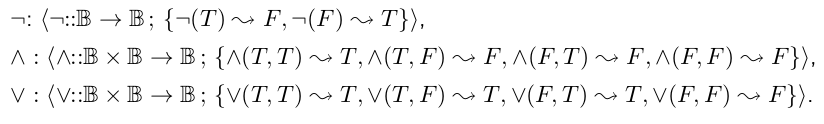
\includegraphics[width=12cm]{computacion.png}
\end{center}
Y computar simplemente significa reemplazar iguales por iguales:
\begin{center}
    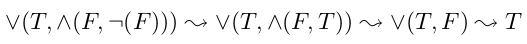
\includegraphics[width=12cm]{computacion2.png}
\end{center}
\end{frame}

\end{document}